% !TEX root = ../main.tex
\newpage
\section{\mywork Mean Field Reductions for undirected graphs}
\subsection{Directed graphs as permutations}
So how can we use the \MFR efficiently when the network is a directed graph with an asymmetrical adjacency matrix? Let's investigate.
\begin{itemize}
\item Sampling $\kinb$ and $\koutb$ from a bivariate distribution requires us to find the marginal distribution of $P$ for $\kinb$, sampling $\kinbi$, and then sampling $\koutbj$ from $P$ while keeping $\kinbi$ fixed. This is a cumbersome process. And what relation would there be between $\kinb$ and $\koutb$?
\item However, if we assume that the marginal distributions for $\kinb$ an $\koutb$ are independent, there is a simplification to be found. We can even assume that the two marginal distributions are identical univariate distributions. 
\item Hence, we can sample $\kinb$ from a univariate distribution and find $\koutb = \permute ( \kinb )$ so that the total number of links remains constant. 
\end{itemize}

This hypothesis can be tested: we assume that $P(\k) = P(\kin) \cdot P(\kout)$ so that $P$ consists of two identical and independent distributions, given by the distributions presented in Chapter \ref{sec:NetworkTopologies}. Then, we sample $\kinb \sim P(\kin)$ and perform a permutation to find all node degrees $\k_j$. The surface given by $P$ and the histogram of $\k_j$ have been plotted in Figure \ref{fig:2Ddistributions}. As we can see, the variates follow the distribution well. 

\begin{figure}[H]
\centering
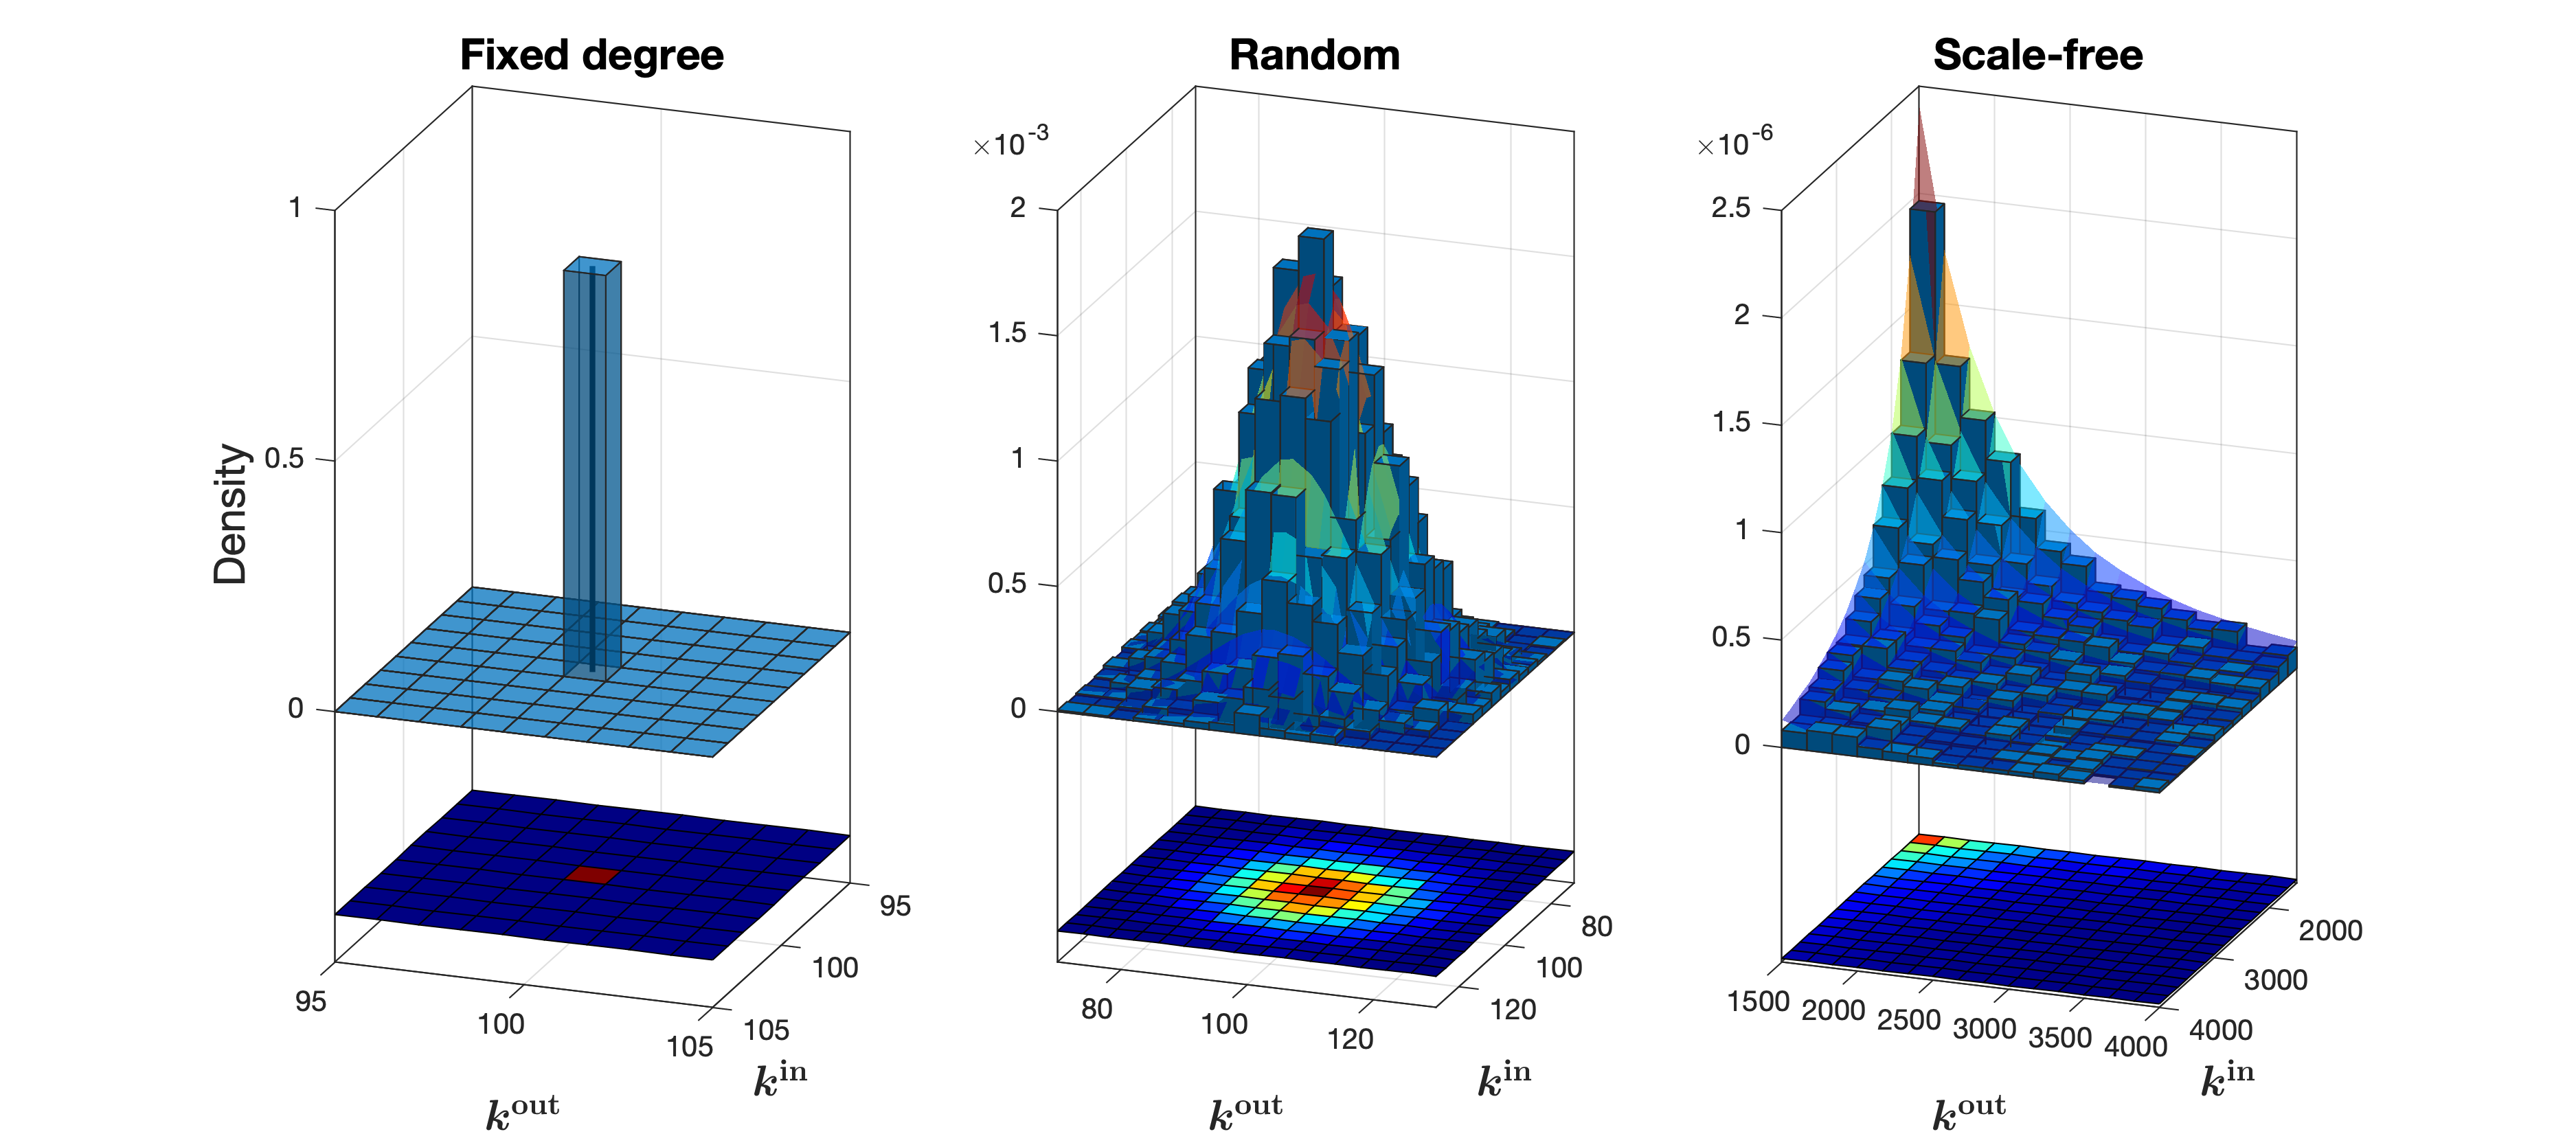
\includegraphics[trim=2.5cm 0cm 2.5cm 0cm, clip=true, width = \textwidth]{../Figures/Distributions/2D.png}
\caption{Bivariate distributions for different network topologies, using 10$^4$ number of samples. The surface given by $P(\k)$ is well approximated by the histogram of variates sampled from a univariate distribution. $\kmean =  2 \times 10^3$ for all topologies, $p \approx 0.2$ for the random network and $\gamma = 4.3$ for the scale-free network.}
\label{fig:2Ddistributions}
\end{figure}


\subsection{Building the adjacency matrix} \label{sec:buildingA}
If we want to simulate the network of theta neurons \eqref{eq:thetaneuronnetworkcurrent} we need to construct the adjacency matrix. We can find an exact solution for $A$ given the degree vectors in \eqref{eq:definekinkoutfromP}. $A_{ij}$ represents a directed graph, but $A_{ij} \neq A_{ji}$ is not a necessary condition. For the elements of $A_{ij}$ we need to find $N^2$ number of variables. We have the following constraints:
\begin{enumerate}
\item The column- and row-sums of $A_{ij}$ must be equal to $\kinb$ and $\koutb$, see \eqref{eq:definekinkoutfromA}. 2$N$ constraints.
\item Self-coupling is mandatory: $A_{ii} = \boldsymbol{1}$. $N$ constraints.
\item The total number of links is constant: $\sum_{i=1}^{N} \kinbi \equiv \sum_{j=1}^{N} \koutbj \equiv \sum_{i,j=1}^{N}A_{i j}$. 1 constraint.
\end{enumerate}
This means that there are $N^2 - (3N + 1)$ variables to find. Once a solution has been found, $A_{ij}$ can be switched with element $A_{ic}$ if $A_{ij} \neq A_{ic}$ and $A_{rj}$ with $A_{rc}$, which yields a new feasible solution. The number of switches one can make is high, and therefore we can simply try a stochastic approach to obtain $A$:
\begin{enumerate}
\item Choose a random row $i \in [1,N]$. $A_{i,i} = 1$, so we need $m = \kinbi - 1$ elements that are 1.
\item Perform $\permute ( \koutbj, j \neq i)$ and therein find the indices $\boldsymbol{\ell}$ of the $m$ first largest elements. 
\item Set $A_{il} = 1 \: \: \forall \: \: l \in \permuteinv (\boldsymbol{\ell})$.
\end{enumerate}
Algorithms that find the largest value in a vector start from the first or the last element. The permutation allows us to find different maxima every time by shuffling the vector.

\begin{figure}[H]
\centering
\begin{subfigure}[b]{0.32\linewidth}
   \centering
  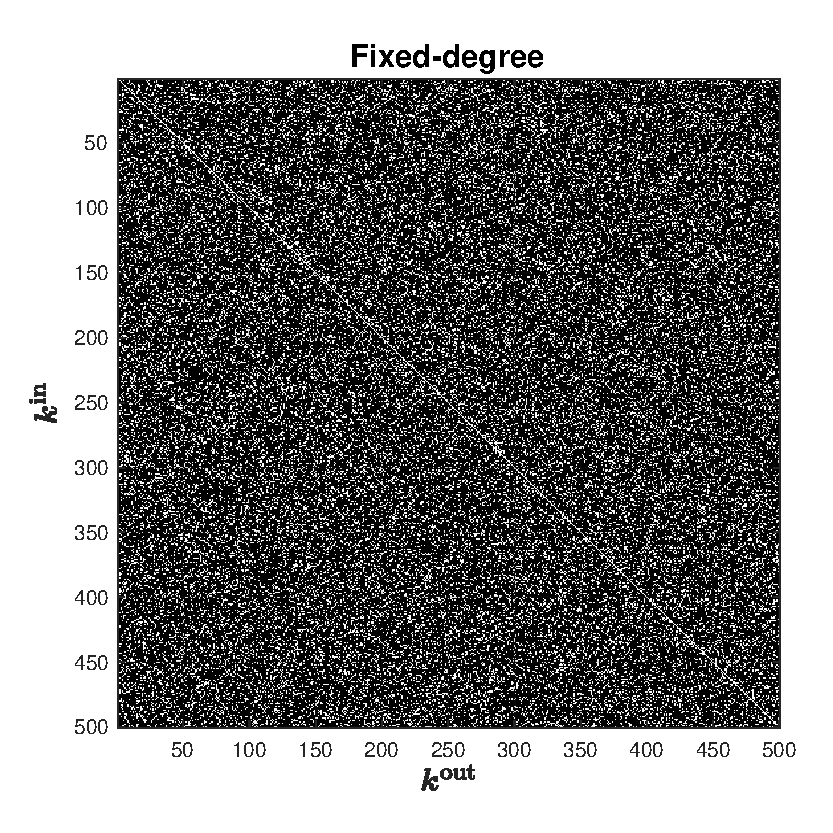
\includegraphics[width=\linewidth, trim={0.5cm 0.5cm 1cm 0.5cm },clip]{../Figures/Adjacency matrices/A_fixeddegree.pdf}
%   \caption{Adjacency matrix for a fixed-degree network.}
 %  \label{fig:A_fixeddegree} 
\end{subfigure} \hfill
\begin{subfigure}[b]{0.32\linewidth}
   \centering
  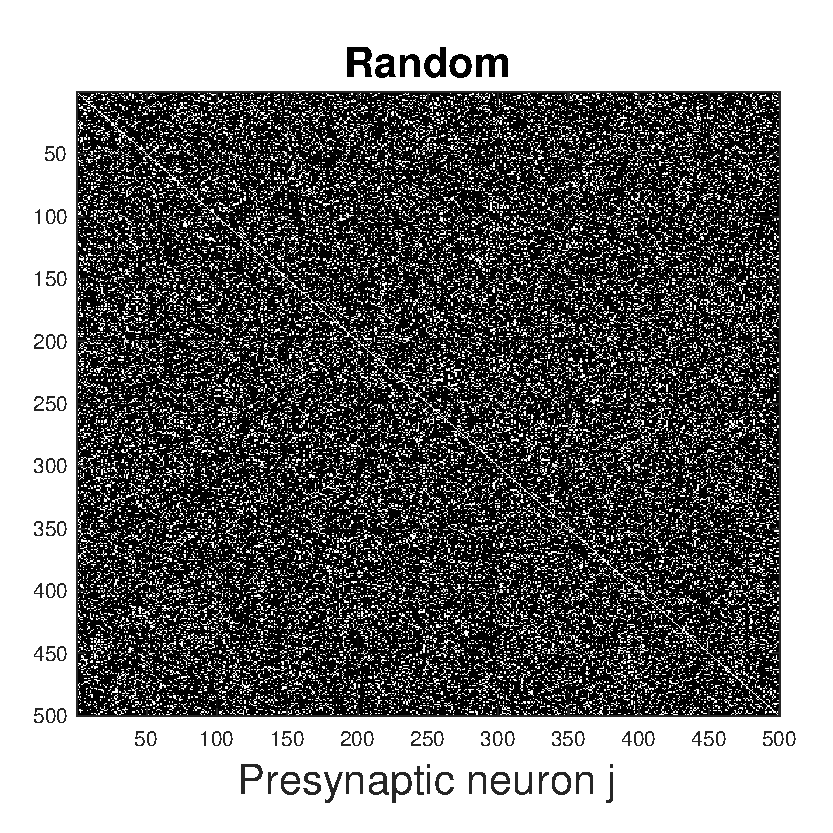
\includegraphics[width=\linewidth, trim={0.5cm 0.5cm 1cm 0.5cm },clip]{../Figures/Adjacency matrices/A_random.pdf}
%   \caption{Adjacency matrix for a fixed-degree network.}
%   \label{fig:MFRPSS}
\end{subfigure} \hfill
\begin{subfigure}[b]{0.32\linewidth}
   \centering
  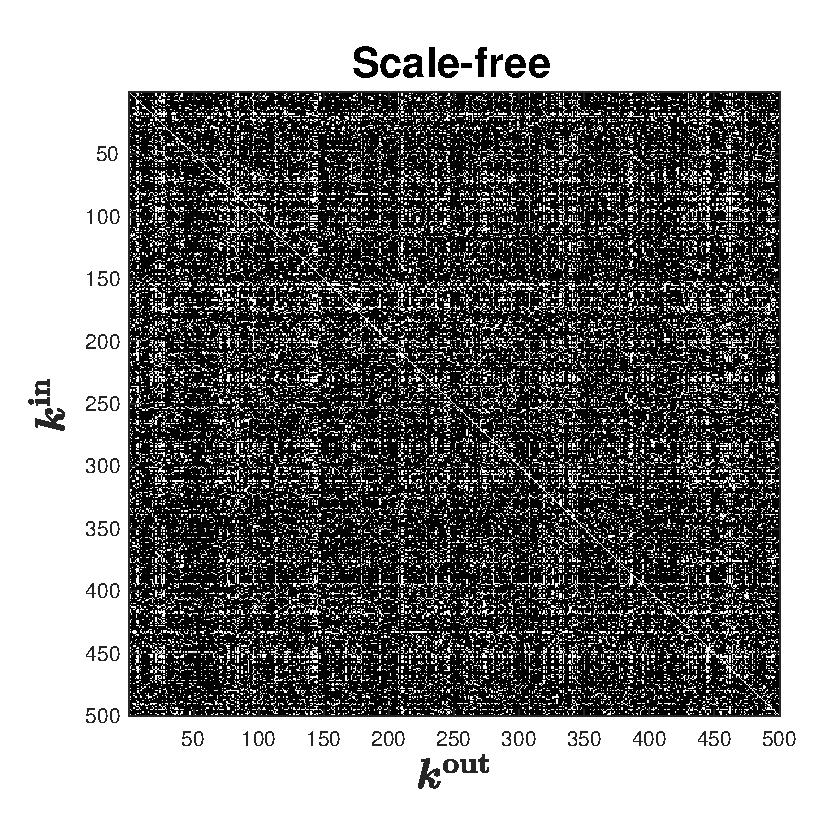
\includegraphics[width=\linewidth, trim={0.5cm 0.5cm 1cm 0.5cm },clip]{../Figures/Adjacency matrices/A_scalefree.pdf}
%   \caption{Adjacency matrix for a fixed-degree network.}
%   \label{fig:MFRCPW}
\end{subfigure}
   \caption{Adjacency matrices for different types of networks with $N$ = 500 and $\kmean$ = 100. We can see how the fixed-degree network is quite homogeneous, while the random network shows some more clustering. The scale-free network has a low number of nodes with a very high degree, which is why we see vertical and horizontal stripes in the adjacency matrix.}
   \label{fig:adjacencymatrices}
\end{figure}

Hence, we can 

\subsection{Fixed-degree networks as a baseline}
\begin{figure}[H]
\centering
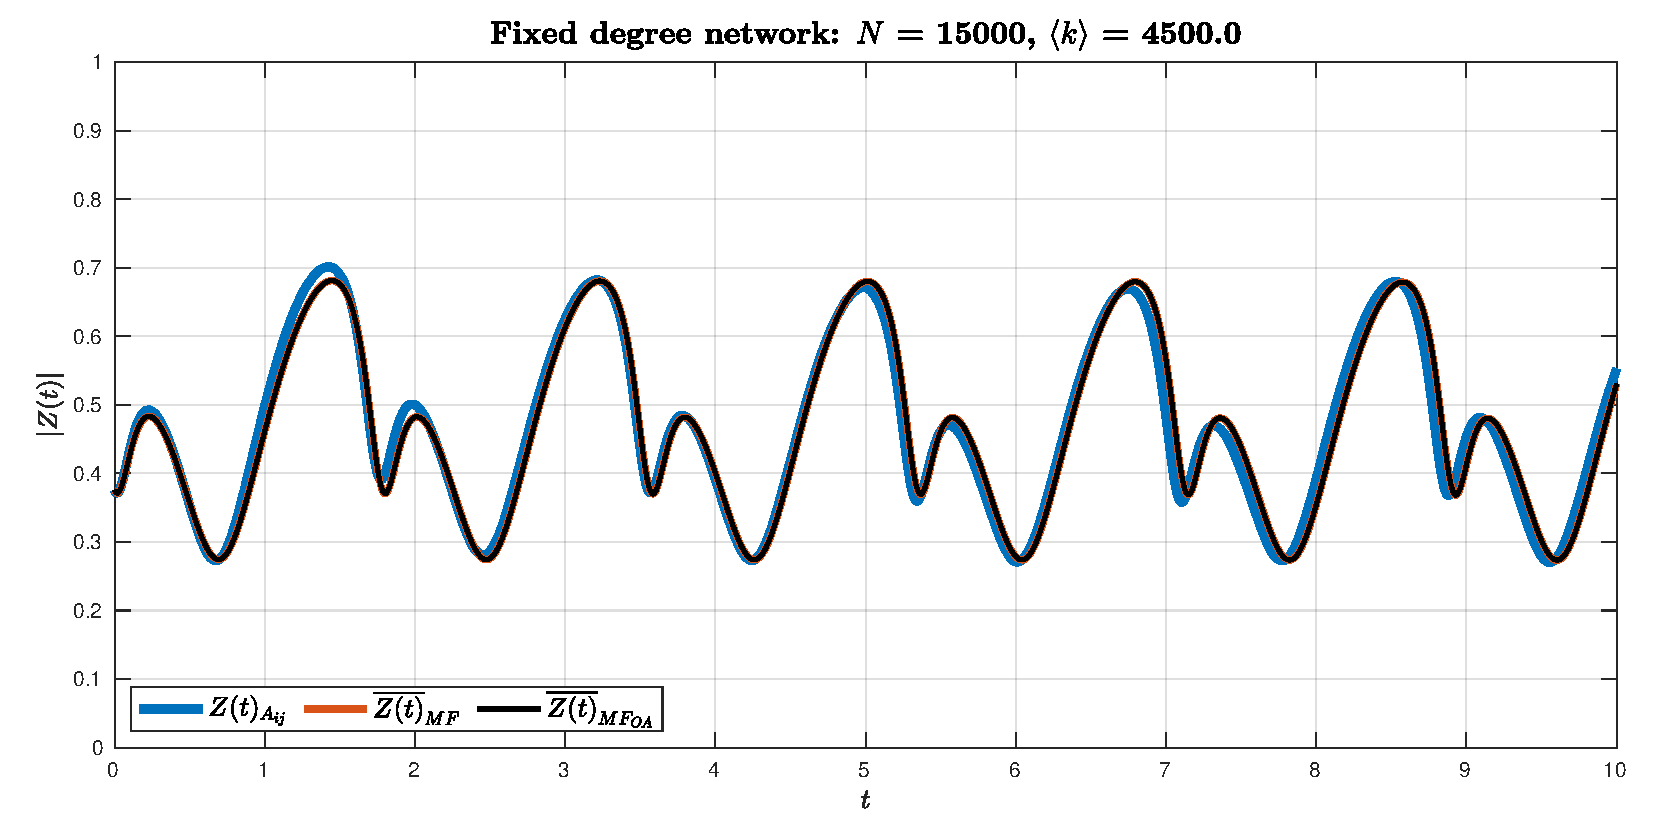
\includegraphics[width = \textwidth]{../Figures/InspectMeanFieldFixedDegree.pdf}
\caption{Comparison}
\label{fig:InspectMeanFieldFixedDegree}
\end{figure}
